Figures \ref{fig:jetson_drone} and \ref{fig:coral_drone} show the fully assembled drones with the Jetson Nano (referred to as the Jetson drone) and Google Coral (referred to as the Coral drone) respectively. The two different companion boards were deliberately chosen in order to provide some comparison between the available systems. Figures \ref{fig:jetson_electronics} and \ref{fig:coral_electronics} show the electronics compartments of the drones. All electronics components in each drone are the same except for the companion boards, camera modules, and the relevant cables. These pictures show the placement of all of the components and their connections, as well as the size difference between the Jetson Nano and the Google Coral. Although the Jetson Nano was ultimately squeezed into the electronics compartment, its large size meant that it required most of the space on the mounting plate. Its fan also extended vertically to nearly the top of the canopy. The consequences of this are discussed in Section \ref{section:jetson_nano_power_consumption_and_form_factor}. By contrast, the Google Coral's smaller form factor (essentially the same as the Raspberry Pi) allows it to fit nicely, leaving even more room for additional components and airflow. The BEC provides a static DC source which generates a magnetic field, and as such it was placed as far away as possible from the compass and GPS receiver (the black case on top of the canopy. The antenna for the telemetry radio extends vertically out of the canopy, while the antennas for the RC receiver extend partially around the circumference of the canopy. The space limitations mean that there is a lot of potential for electrical and radio interference among the components. However, the different radio bands used by the components, as well as the little available physical separation that was achieved through the placement of the components, provide adequate performance during tests.

\begin{figure}
    \begin{subfigure}[b]{0.48\textwidth}
        \centering
        \includegraphics[width=\textwidth]{images/jetson_drone.JPG}
        \caption{The Jetson drone.}
        \label{fig:jetson_drone}
    \end{subfigure}
    \begin{subfigure}[b]{0.48\textwidth}
        \centering
        \includegraphics[width=\textwidth]{images/coral_drone.JPG}
        \caption{The Coral drone.}
        \label{fig:coral_drone}
    \end{subfigure}
    
    \begin{subfigure}[b]{0.48\textwidth}
        \centering
        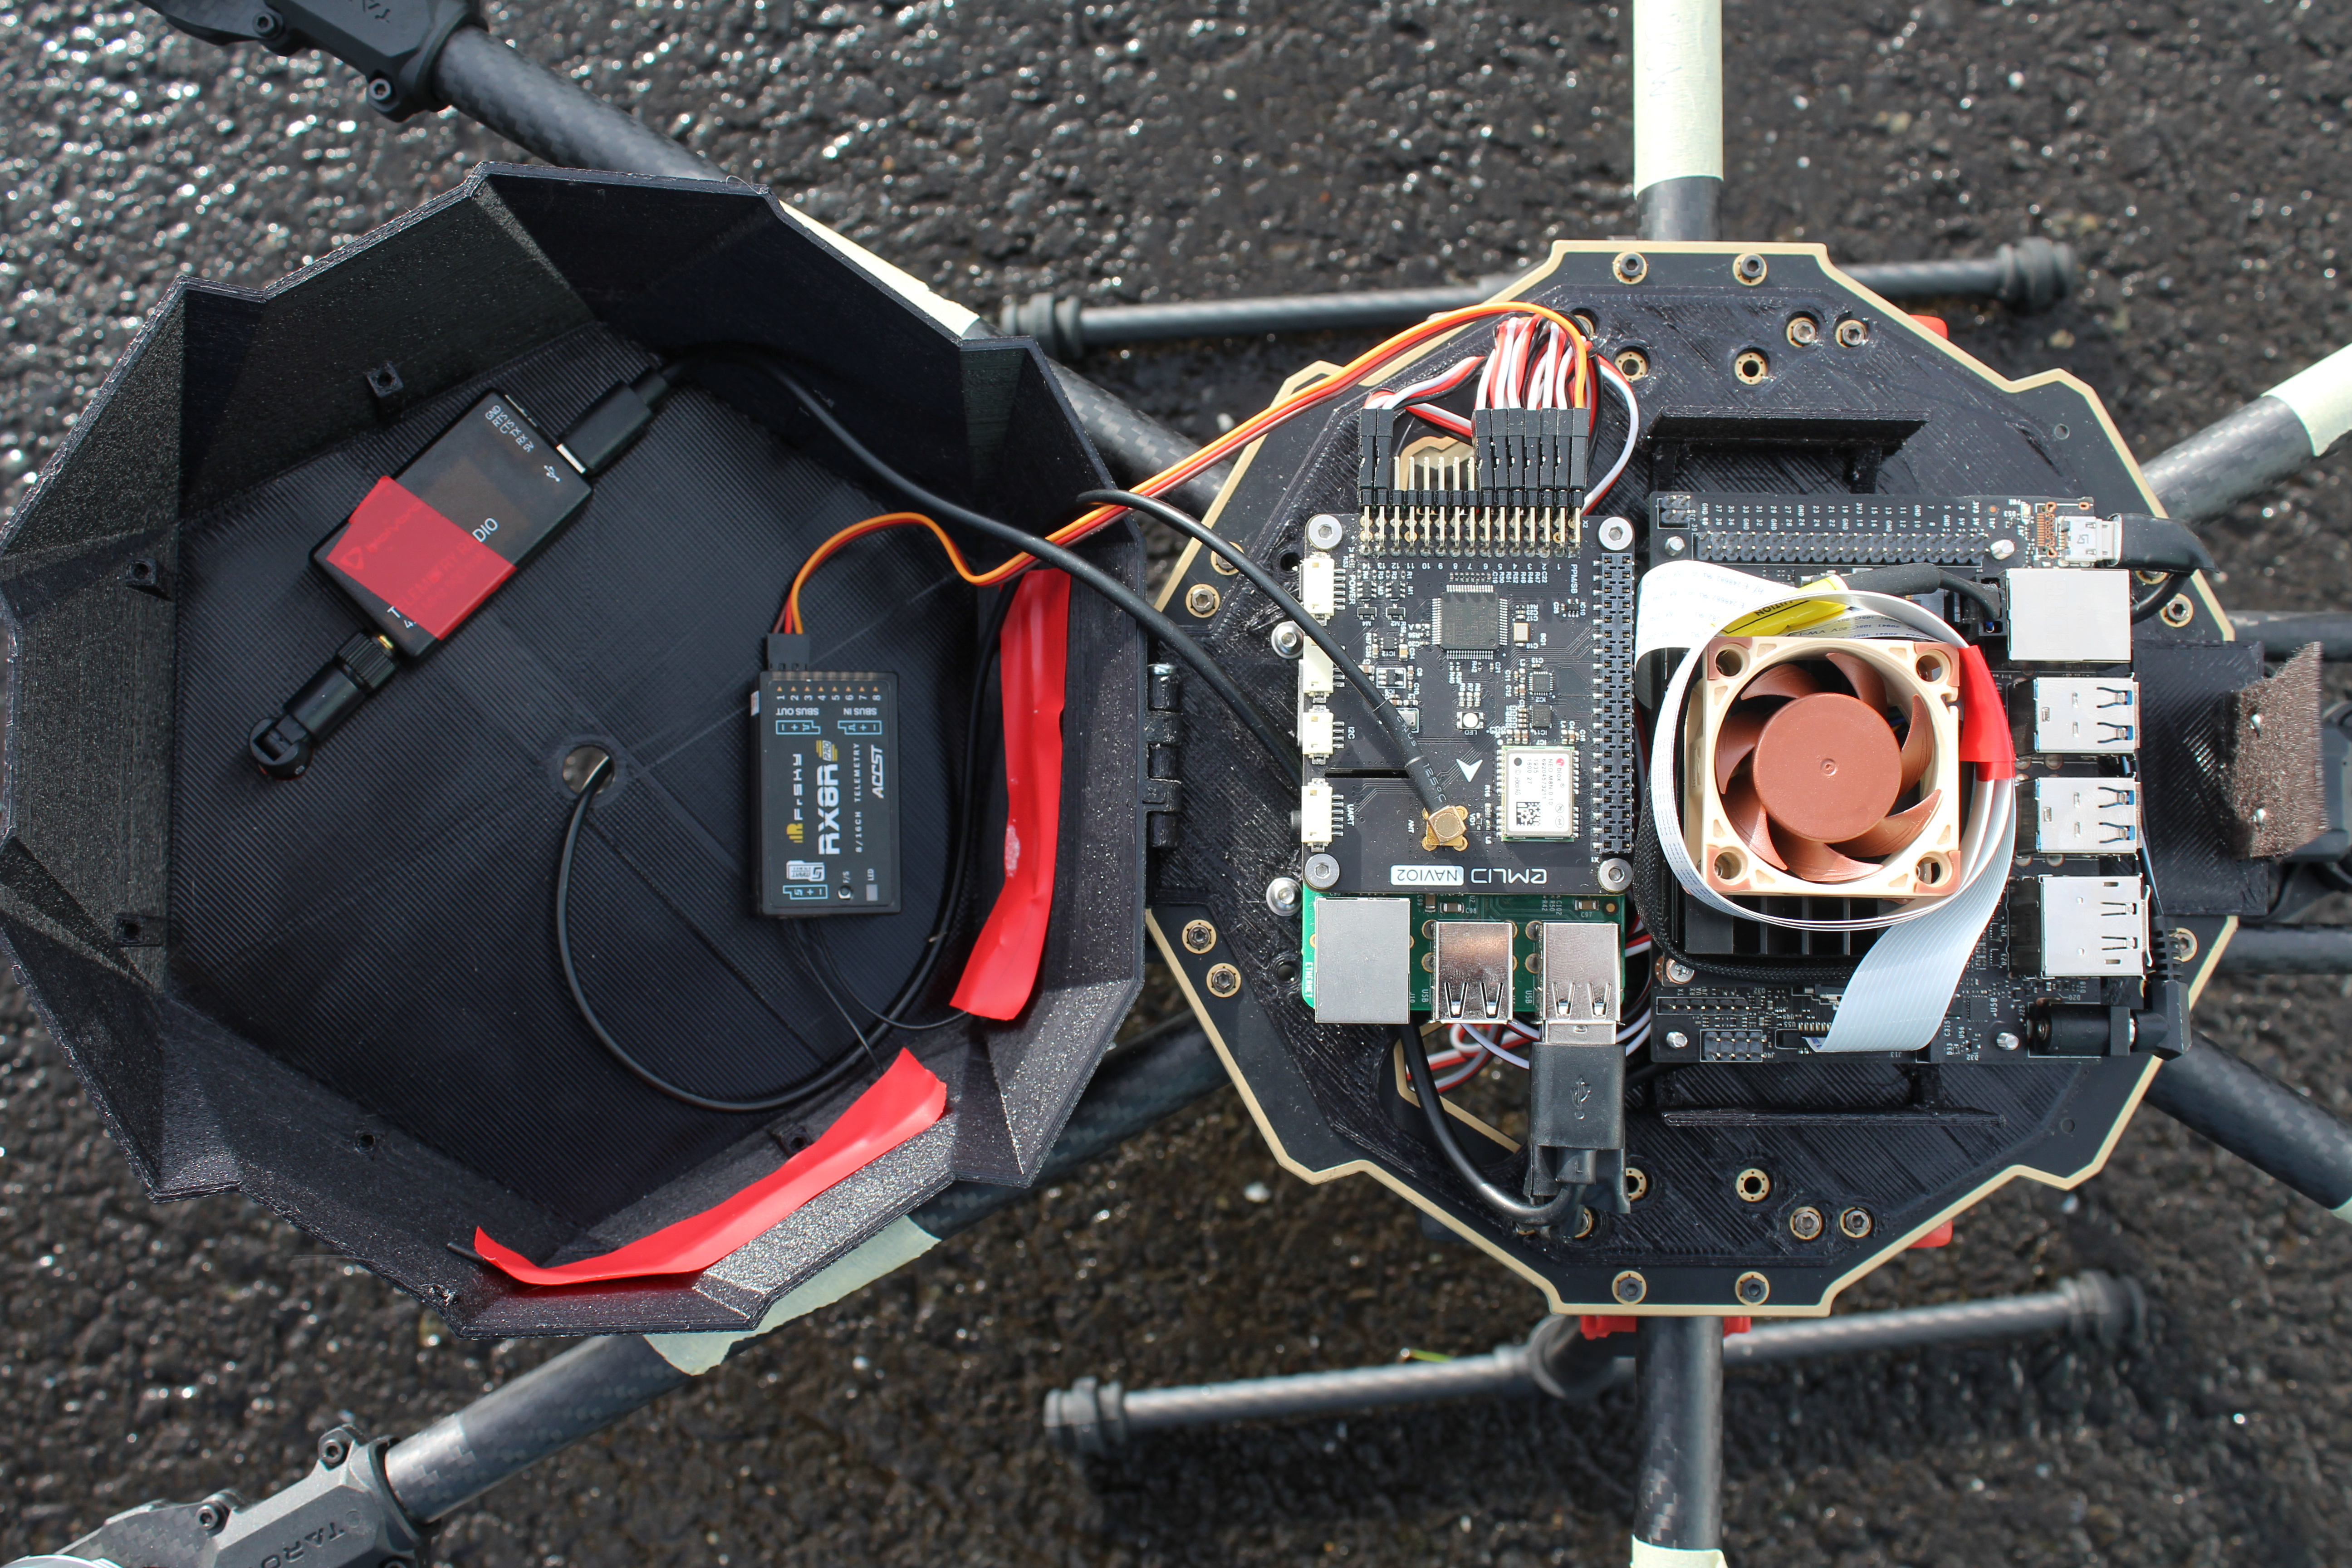
\includegraphics[width=\textwidth]{images/jetson_electronics.JPG}
        \caption{The Jetson drone's electronics compartment.}
        \label{fig:jetson_electronics}
    \end{subfigure}
    \begin{subfigure}[b]{0.48\textwidth}
        \centering
        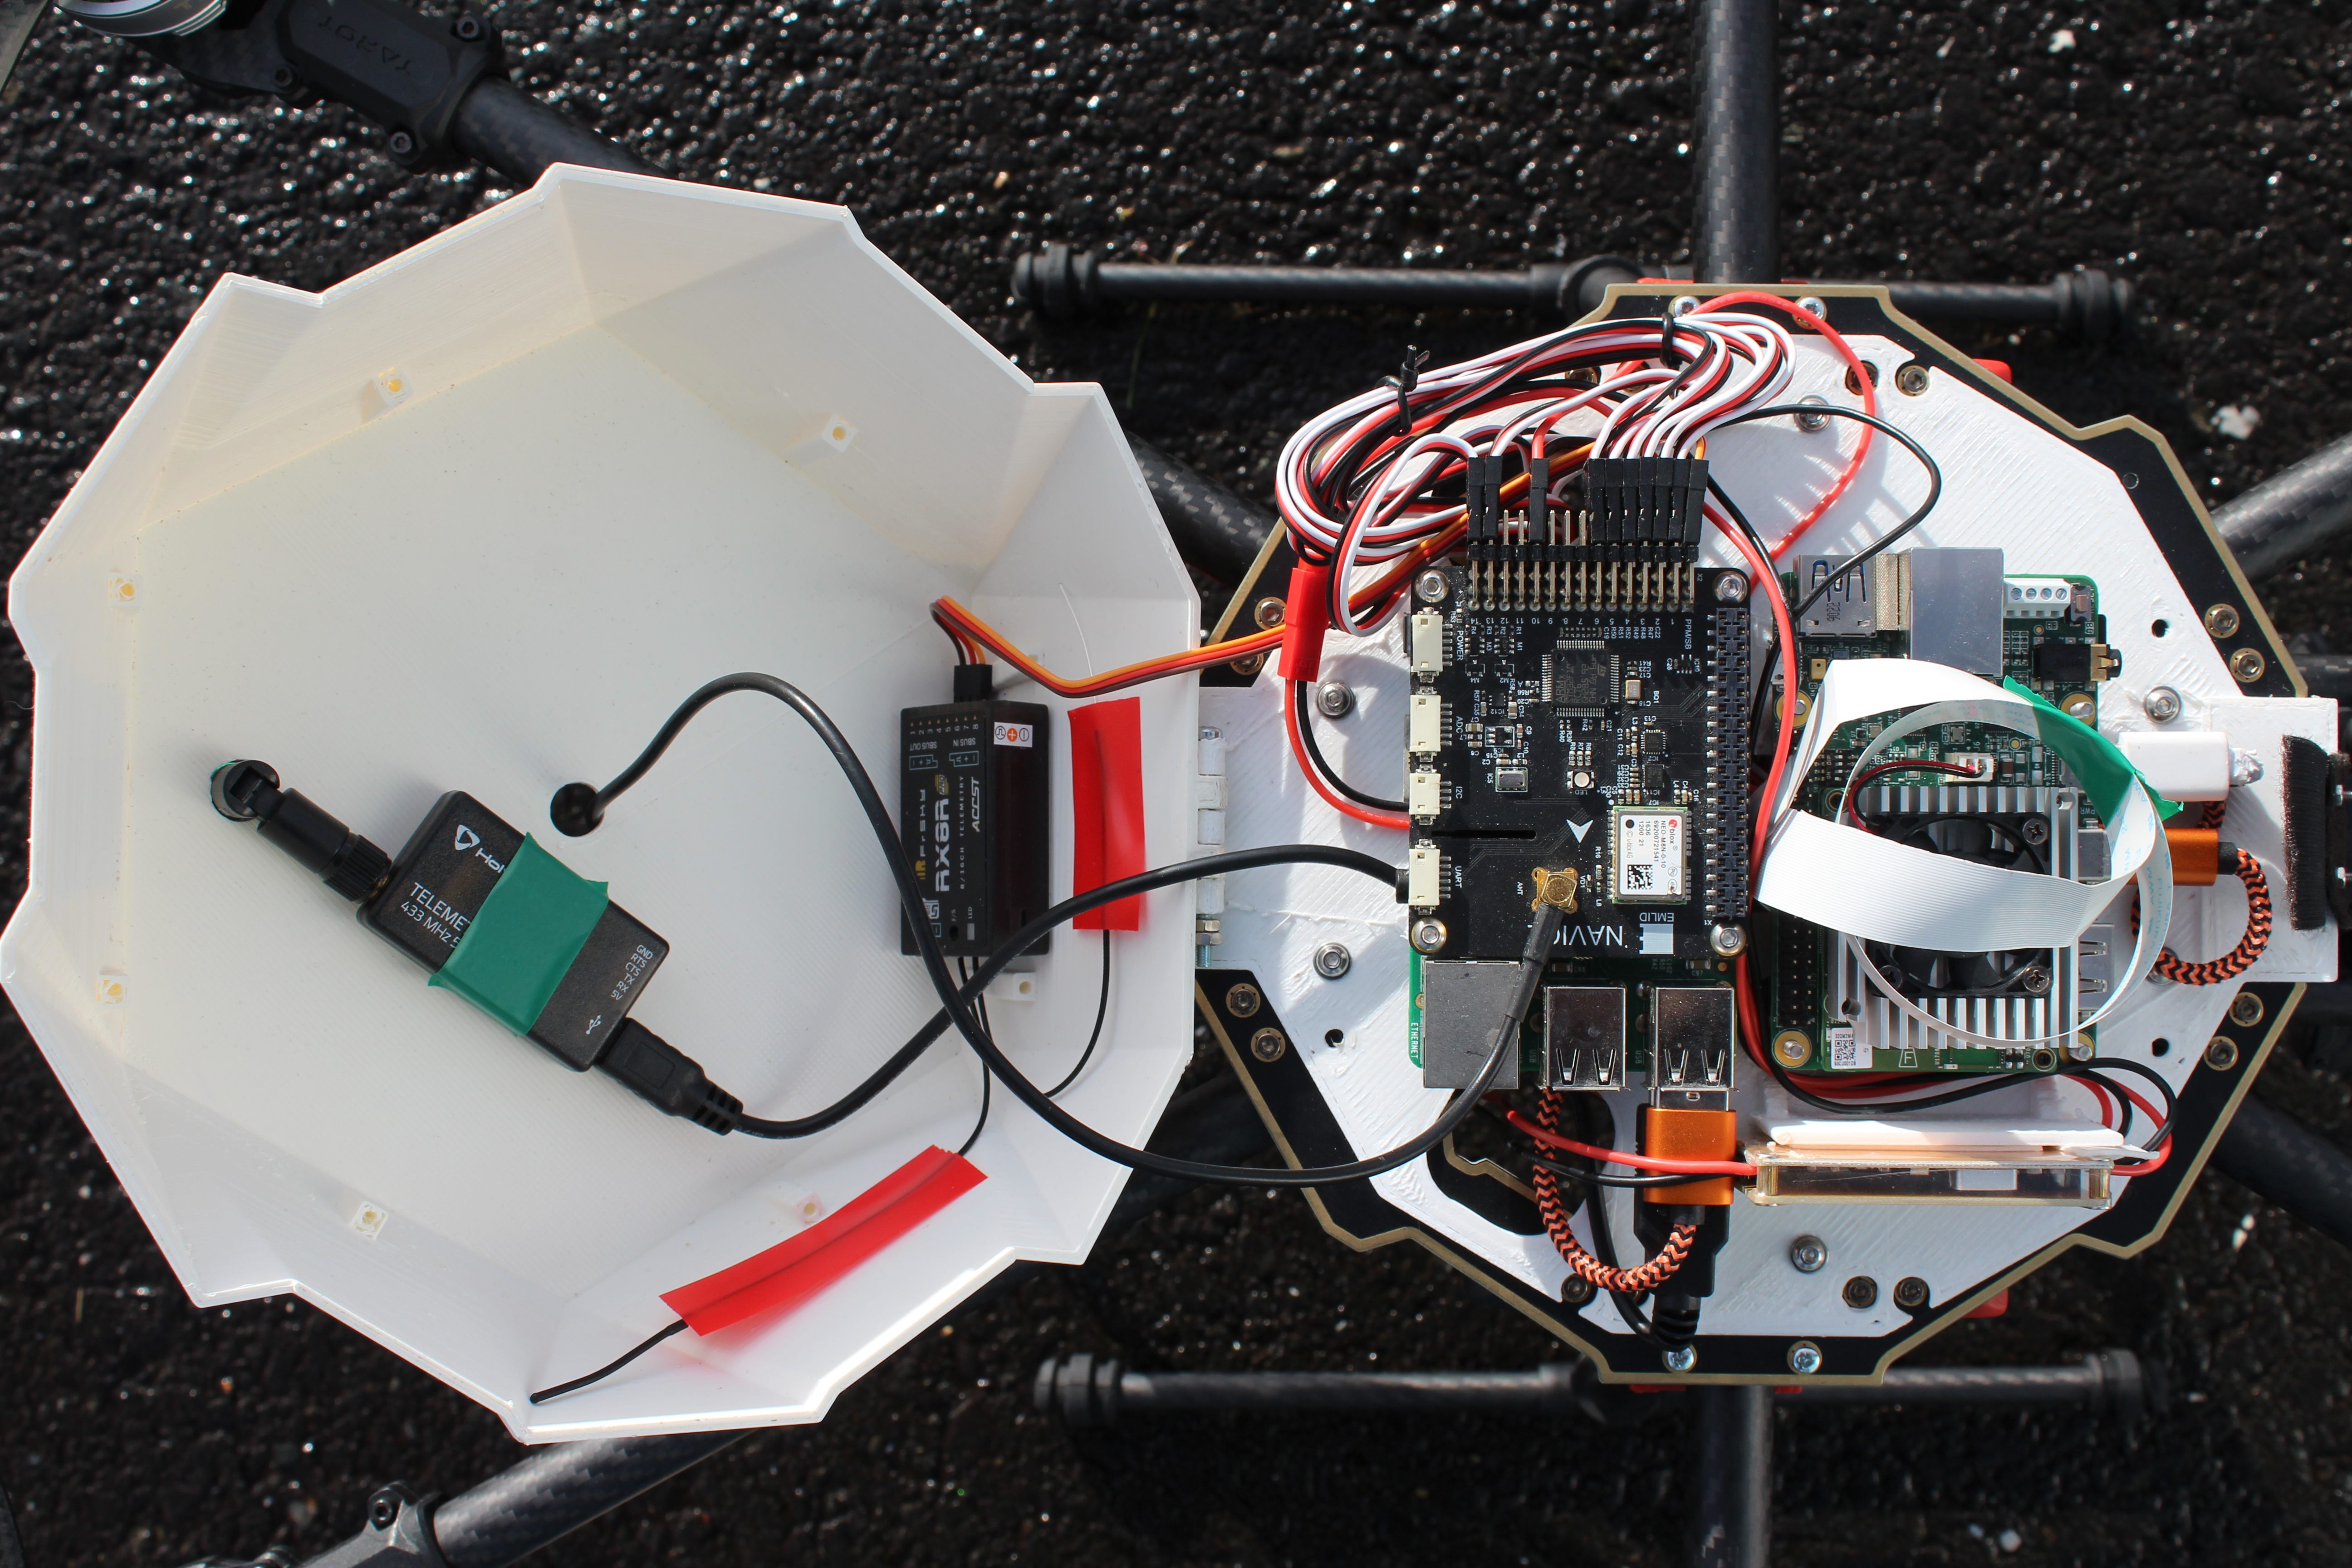
\includegraphics[width=\textwidth]{images/coral_electronics.JPG}
        \caption{The Coral drone's electronics compartment.}
        \label{fig:coral_electronics}
    \end{subfigure}
    
    \caption{The assembled drones and their electronics compartments.}
    \label{fig:drone_pictures}
\end{figure}